\section{Related Works}

\subsection{Light Fields and Novel View Synthesis}
In the fields of computer graphics and computer vision, novel view synthesis refers to the problem of, given a relatively small set of model images from different camera positions, generating an image representing the model from a point of view different from the input model images. The main advantage of this approach is to avoid the computationally expensive tasks of creating a 3D model, texturing, and rendering. In traditional computer vision, this task was performed by manipulating the input images through techniques such as flow-based interpolation and mosaic compositing. The main drawbacks of these techniques are the large amount of input images necessary to obtain quality results, and the need for significant overlap between model images \cite{Avidan97}.

One idealized concept in vision that would allow the representation of a scene from any point and any orientation is the plenoptic function. A three-dimensional color lightfield is defined by the 6-dimensional plenoptic function $P(\theta, \phi, \lambda, x, y, z)$. This function $P$ denotes the light intensity with wavelength $\lambda$ passing through the point $(x, y, z)$ through a ray direction parameterized by the spherical coordinates $(\theta, \phi)$ \cite{Landy91}. If the plenoptic function corresponding to an environment is known at all points and viewing directions, then the task of generating a novel view becomes as trivial as performing an angular integration at all camera pixel positions over all incident rays \cite{Martinez-Corral:18}.

However, being an idealized concept, it cannot be completely specified for a natural scene as it would require the measurement of light intensity at infinite points in space from infinite directions, which is impossible in practice. However, multiple views of a model can help build an approximation of a discretized plenoptic function, and it hints to its ability to be used as an implicit representation of an environment, which will be later leveraged by Neural Radiance Fields to encode the illumination of a scene.

\subsection{Structure from Motion}
Before diving into an analysis of modern approaches to model reconstruction from 2D images, it is worth going over the Structure from Motion (SfM) algorithm, which serves as a starting point for all of the methods I will discuss later. The main problem this algorithm solves is inferring the 3D structure and motion of objects from the 2D transformation of their projected images when no other spatial information is given. The algorithm is based on the "structure from motion" theorem, which states that, given 3 orthographic projections, the structure of 4 non-coplanar points in space can be recovered \cite{ullman79}. For modern applications, the problem actually becomes retrieving 3D information about a scene from a set of unordered 2D images. COLMAP \cite{schoenberger2016mvs,schoenberger2016sfm} is a pipeline implementing the SfM algorithm for this purpose and is used as an incipient step by all environment reconstruction models that I will present in the later sections. 

The COLMAP algorithm is divided into two stages: Correspondence Search and Incremental Reconstruction. The \textbf{Correspondence Search} step takes as input the set of unordered images and outputs a set of geometrically-verified image pairs and a graph of image correspondences. First, for each image, a set of geometrically invariant features is generated, which will serve as a basis for finding correspondences between images in the initial set. Then, by leveraging these feature descriptors, the algorithm finds images that see the same parts of the scene. This first mapping is only computed based on appearances, so there is no guarantee that the features actually map the same scene point. In order to verify this match, the algorithm tries to find a homography that maps the features between the two images. If enough features match after applying the transformation to one of the image planes, then the image correspondence is added to the scene graph. The second stage, \textbf{Incremental Reconstruction}, takes as input the scene graph and outputs estimated poses for each image and a point cloud reconstruction of the scene. SfM initializes the model from a two-view reconstruction, which has to be carefully selected, as it can heavily influence the quality of the result. Then, in an iterative manner, more images can be added to the model. The criterion for selection is that a newly registered image must observe existing points in the model. This allows to determine camera parameters relative to the existing model, and also to triangulate the positions of the new feature points the image adds to the model. However, new points can be triangulated only when they are seen from two distinct perspectives. Even though registration and triangulation are highly correlated, incremental errors from both processes result in the reconstruction drifting, so a bundle adjustment step is necessary. This is a non-linear refinement of camera parameters and feature point parameters in order to minimize the reprojection error. An overview of the complete pipeline can be seen in figure \ref{fig:sfmpipeline}.

\begin{figure}[H]
    \centering
    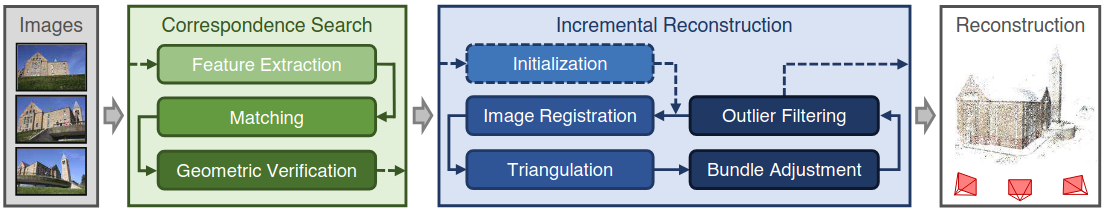
\includegraphics[width=0.7\linewidth]{figures/sfm.png}
    \caption{Complete SfM pipeline. Taken from \cite{schoenberger2016sfm}.}
    \label{fig:sfmpipeline}
\end{figure}

After this pipeline is executed, each input image will have associated a pose and camera intrinsics which approximate the relative position of the camera where the image was taken. Moreover, a reconstructed point cloud is provided, which can serve as a starting point for environment reconstruction algorithms. 

\subsection{Neural Radiance Fields}

The first NeRF model was published in 2020, and since then a lot of variations have emerged in an attempt to address some of its issues and improve its performance metrics. I will first go over the initial implementation, as it serves as a base for its follow-ups and illustrates the fundamentals of neural scene encodings.
\subsubsection{NeRF}

The main idea behind NeRF is to encode a static scene using a fully connected deep neural model \cite{mildenhall2020nerf}. The input of the model is a five-dimensional vector representing a position in space $\textbf{x}$ and a viewing direction $\textbf{d}$ and outputs the volume density at that point $\sigma$ and the view-dependent radiance $\textbf{c}$. This is quite similar to the formulation of the plenoptic function of a light field, however, the neural model can only provide an approximation of it through the following function $F_\Theta : (\textbf{x}, \textbf{d}) \rightarrow (\textbf{c}, \sigma) $. Generating a novel view is done by querying 5D points along camera rays and accumulating the density and emitted color, just like any volumetric renderer. Since this raymarching method for rendering the images is fully differentiable, gradient descent can be used to optimize the model by minimizing the difference between the reference images and the renders obtained from querying the model. An overview of the training process can be seen in figure \ref{fig:nerf}.

\begin{figure}[H]
    \centering
    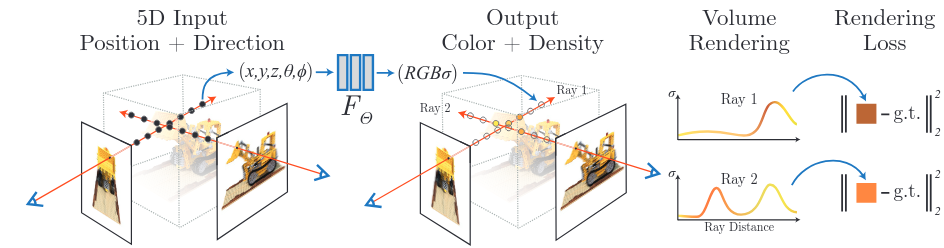
\includegraphics[width=0.7\linewidth]{figures/nerf.png}
    \caption{NeRF training process, from \cite{mildenhall2020nerf}.}
    \label{fig:nerf}
\end{figure}

Even though the neural network is used as a generic function approximator, it tends to bias towards favoring lower frequency information. To address this issue, the input query points are first mapped into a higher dimensional space using higher frequency functions, thus creating a positional encoding, which promotes the learning of high-frequency features. In order to optimize the ray marching component, two models are trained for the same scene, one "coarse" and one "fine". The coarse model is sampled first to determine regions that require more sampling in order to allocate more sampling points to areas that are expected to have more impact on the final render. Using these strategies, they were able to surpass in terms of quality existing volumetric scene reconstruction implementations.

\subsubsection{Mip-NeRF}
An immediate follow-up to the original implementation of NeRF is Mip-NeRF \cite{barron2021mipnerf}. It addresses the multi-resolution issues in NeRF, where a model can be rendered with high quality only when the scale is the same as that of the training images. This happens because of the ray sampling strategy, where rays are evaluated at individual points, so as the model gets further away from the camera, the volume gets more sparsely sampled and aliasing artifacts start to appear. Also, for synthetic scenes, the reference cameras are all at the same distance from the model, so a single-resolution model cannot solve a multi-resolution problem efficiently. The solution to this issue is inspired by the mipmapping algorithm for texture sampling, where lower-resolution textures are prefiltered, and then can be interpolated between levels to obtain the desired resolution. To achieve this effect, the ray sampling is changed from point sampling to volumetric sampling through integrated positional encodings. Computing and sampling a cone around a ray is computationally expensive, so around each sample point, a multivariate Gaussian is fitted in order to approximate the sampling volume. Figure \ref{fig:mipnerf} shows the difference in model sampling between the reference NeRF implementation and Mip-NeRF. As the sample point gets further away from the camera, the sampled volume gets bigger. This can be achieved by shrinking the high-frequency positional encodings, thus sampling the lower-frequency features, which achieves the same effect as prefiltering. The advantage of this approach is that the quality of the high-resolution renders remains completely unaffected, while lower-resolution renders become more photorealistic. This allows zooming into models without losing quality and also seamlessly transitioning between different levels of detail.

\begin{figure}[H]
    \centering
    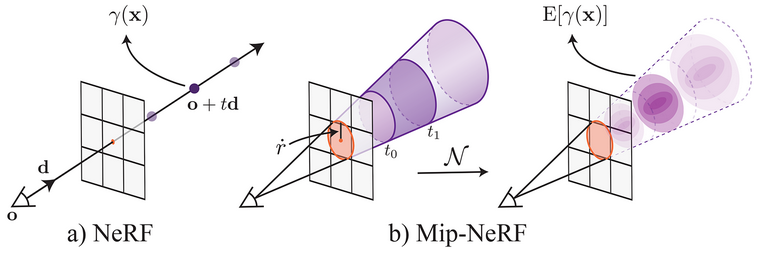
\includegraphics[width=0.6\linewidth]{figures/mipnerf.png}
    \caption{Differences in model sampling between NeRF (left) and MipNeRF (right), from \cite{barron2021mipnerf}. }
    \label{fig:mipnerf}
\end{figure}

\subsubsection{FastNeRF}
Besides addressing the image quality, some implementations try to improve the rendering speed of the original NeRF, which is far from being able to be used in real-time rendering. By building a cache structure of the radiance map represented by the model and querying it instead of the neural network, FastNeRF achieves a roughly 3000x increase in rendering performance without sacrificing quality \cite{garbin2021fastnerf}. The main idea of the cache is to take as input the position and orientation vectors and produce the estimated density and illumination values in a roughly constant time. However, building a cache for a 5-dimensional input is very taxing in terms of required space, and even moderate resolutions would require unreasonable amounts of storage space. In order to avoid the issues of high polynomial increase of storage requirements with resolution, the authors propose a separation of the model into a position cache and an orientation cache.  A simplified representation of the architecture can be seen in figure \ref{fig:fastnerf}.

\begin{figure}[H]
    \centering
    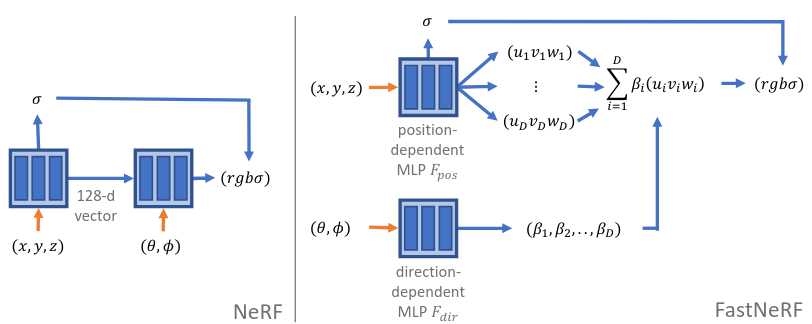
\includegraphics[width=0.6\linewidth]{figures/fastnerf.png}
    \caption{Reference NeRF model (left) and FastNeRF split architecture (right) \cite{garbin2021fastnerf}.}
    \label{fig:fastnerf}
\end{figure}

The estimated density is only a function of position, but the radiance depends on both position and viewing direction. To overcome this parameter coupling, the position-queried model produces a set of deep radiance maps for each point in space, and the direction-based model produces a set of weights corresponding to each of the deep irradiance maps. This approach is similar to the use of spherical harmonics to estimate directional illumination. By taking the dot product between the deep irradiance map and the weight vector, the local irradiance can be estimated while also taking into account the viewing direction. By building two separate caches following this strategy, the required storage space can be reduced to reasonable values. Also, by adjusting the dimension of the cache, the tradeoff between quality and storage can be balanced depending on the application. However, the main drawback of this implementation is that in order to achieve comparable quality metrics to the original NeRF, the model size is drastically increased, but in turn, enables the use of NeRF for real-time scenarios. 

\subsubsection{Mip-NeRF360}
All of the NeRF methods presented above are trained and evaluated on scenes containing one central model and a black background. This is because these models are confined to a bounded volume for their representation and cannot fit large scenes efficiently, as the background could be very distant. Moreover, the disparity between the detail in the foreground and the background introduces floating artifacts in the scene, as the representation becomes ambiguous in areas that are seen by few camera positions. The architecture of Mip-NeRF360 proposes a solution to this issue \cite{barron2022mipnerf360}. To address the first problem of the scene being unbounded, the authors propose a reparameterization of the coordinate vector through a strategy similar to an Extended Kalman filter. In this approach, the coordinates inside the unit sphere remain unchanged, and the rest of the coordinates outside the unit sphere are remapped to the sphere of radius 2. This means that also the volumetric Gaussians used for sampling but Mip-NeRF will get distorted as the scene elements get further away from the center point of the scene, as can be seen in figure \ref{fig:mipnerf360-scene}.

\begin{figure}[H]
    \centering
    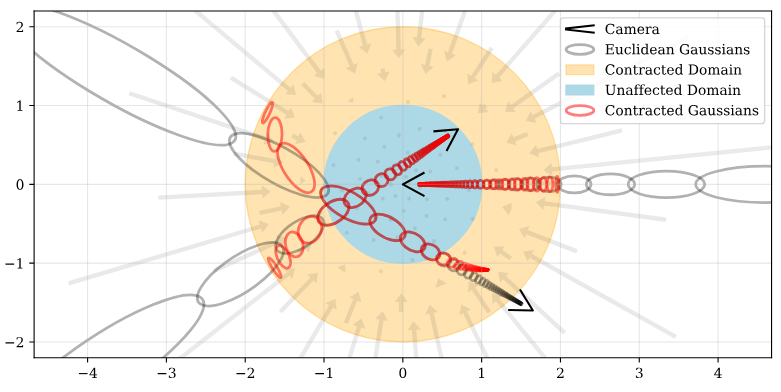
\includegraphics[width=0.5\linewidth]{figures/mipnerf360-scene.png}
    \caption{Mip-NeRF360 scene compression \cite{barron2022mipnerf360}.}
    \label{fig:mipnerf360-scene}
\end{figure}


The original Mip-NeRF runs both coarse and fine evaluations along the rays using the same MLP, where zones of interest are determined by the coarse sampling and they determine where the finer sampling should be performed. However, this is wasteful in terms of computation time, since only the density is needed in the coarse sampling. This new architecture introduces a second MLP which acts as a proposal model, and which only outputs a density distribution along the ray in order to determine the finer sampling of the actual NeRF MLP. This can be thought of as an online distillation method since both models are trained together. The proposal model is not trained directly, as it is only constrained that the density histogram it emits is consistent with the histogram of the NeRF MLP since they represent the density distribution along the same ray. The last improvement proposed by the authors for this model is the introduction of a regularization step which is applied to the weighted density distribution along each ray. In short, the regularizer is trying to minimize the total distance between pairs of sequential points along the ray, as shown in figure \ref{fig:360grads}. This minimum can be achieved only when the weights are 0, which means that the ray would be empty. However, in the case of non-empty rays, it is minimized by consolidating the weights into a region as small as possible. This in turn has the effect of removing floating artifacts, which are introduced by distant elements of the scene by effectively "pulling" them towards their correct position. 

\begin{figure}
    \centering
    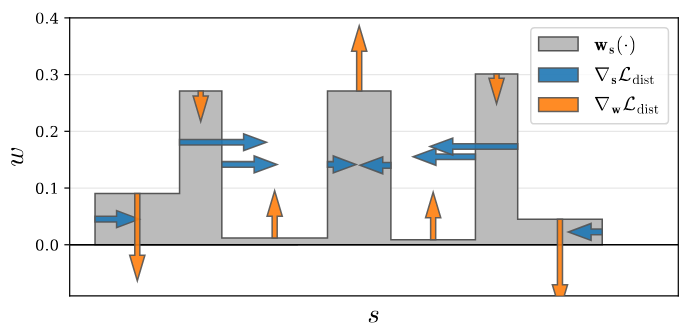
\includegraphics[width=0.6\linewidth]{figures/360-gradients.png}
    \caption{Regularization function and its gradients \cite{barron2022mipnerf360}.}
    \label{fig:360grads}
\end{figure}

Using these 3 improvements, Mip-NeRF360 can efficiently model unbounded scenes and greatly surpasses the models preceding it in terms of visual quality.

\subsection{Plenoxels}
Plenoxels is a photorealistic view synthesis system that adopts the idea of differentiable rendering from NeRF, but it attempts to encode a scene representation without an MLP \cite{yu_and_fridovichkeil2021plenoxels}. Instead, this model uses a sparse 3D grid of voxels called plenoptic volume elements, which store spherical harmonic information and density on their vertices. Then, the color and density at any arbitrary point can be determined by trilinear interpolation of the values at the corners of the voxel containing said point. This allows for simple rendering based on raycasting, similar to any other volumetric renderer. Using this interpolation approach, the model can define a continuous plenoptic function throughout the whole model. During model optimization, the spherical harmonic coefficients and opacities are updated with respect to the mean square error between the rendered image and the reference images, as well as using a total variation regularization term. Optimization is done in a coarse-to-fine manner. Going over the coarse voxel grid, unnecessary voxels are pruned and the voxels in detailed areas are subdivided, then the optimization is performed on the finer grid. The total variation term in the cost function has the purpose of removing high-frequency noise in the reconstruction and is balanced with the image quality metric through the regularization weight $\lambda_{TV}$. Figure \ref{fig:plenoxel} shows an overview of the plenoxels scene optimization pipeline.

\begin{figure}[H]
    \centering
    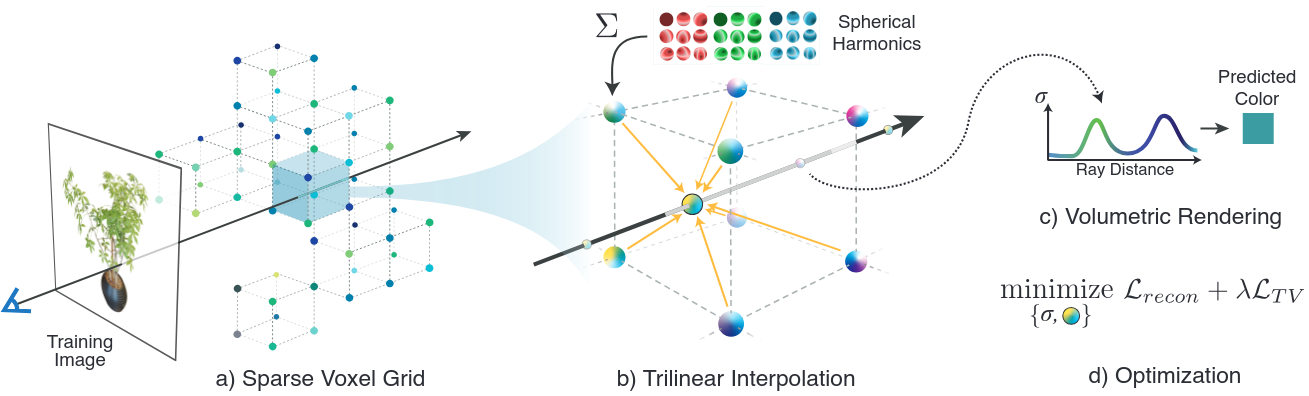
\includegraphics[width=0.7\linewidth]{figures/plenoxels.png}
    \caption{Plenoxels model optimization pipeline \cite{yu_and_fridovichkeil2021plenoxels}.}
    \label{fig:plenoxel}
\end{figure}

This model can achieve up to 100x improvement in training time compared to typical NeRF implementations while maintaining similar image quality metrics, and with minimal changes can be adapted to unbounded scenes. For real unbounded scenes, the sparse volume is surrounded by a set of background spheres, which in turn represent sparse voxel grids that will model the background, interpolating both within each sphere and between adjacent spheres.

\subsection{Splatting for Volume Rendering}
Traditional volumetric rendering techniques such as ray casting, which is the primary rendering method in NeRF-like models, offer very good quality as they evaluate the path of multiple rays through the volume and accumulate light information in a realistic manner, they are very compute-intensive and sometimes not fit for real-time applications. The first approach of accelerating volume rendering through a forward-mapping algorithm was proposed by Westover L. in 1989 \cite{westover89splatting}. In order to accelerate rendering, the initial volume is sampled along a regular grid at the desired resolution. These samples are then considered particles that emit or absorb light and influence the final image. Line integrals are computed across each particle to determine its footprint on the camera plane. This removes the issue of raycasting, as now instead of determining which sample each pixel "sees", the problem becomes determining which pixels each sample influences, which reduces the complexity since volume samples are considered to be simple volumetric primitives. Reconstructing a continuous signal from discrete signals is done by convolution with a reconstruction kernel. For band-limited signals, a perfect reconstruction can be achieved using the \textbf{sinc} function as a convolution kernel. However, the volume samples have a limited volumetric span, and the sampling frequency in the initial grid is dictated by performance requirements so it may not follow the Nyquist-Shannon sampling theorem, so the samples are convoluted with discs whose properties vary in a Gaussian manner. After the image signal is reconstructed from the discrete samples, the color on each pixel is blended using a back-to-forward or forward-to-back traversal over the samples that influence it. This way, rendering volumetric data can be performed significantly faster, albeit at a cost to image quality. 

Even though it went through numerous changes, splatting has become popular recently as an alternative to NeRFs, where the scenes are represented explicitly through Gaussian primitives. Even though the current implementation follows the general direction of the original, it is no longer a method for approximating known volumetric data for the purpose of rendering, but the splats themselves are the base representation of the data. In the following subchapters, I will go over the original implementation of Gaussian splatting for novel view synthesis, as well as some variations of it that are relevant to my work.

\subsubsection{3D Gaussian Splatting for Real-Time Radiance Field Rendering}
Radiance Field methods have brought many advancements to environment reconstruction by encoding scenes through a Multi-Layer Perceptron network. However, these methods sacrifice rendering speed for quality, especially in complex or unbounded scenes, as continuously evaluating the neural network during rendering significantly limits frame times. However, an alternative to this is brought by 3D Gaussian Splatting models \cite{kerbl3Dgaussians}, which represent the scene explicitly through Gaussian primitives, which allows for achieving real-time rendering speeds. This implementation provides a methodology of using 3D Gaussians to represent a continuous radiance field, optimizing the scene, and rendering the scenes using a differentiable visibility-aware process that allows it to achieve real-time frame times. 

Just like the NeRF models, this implementation also starts with processing the input images through a Structure from Motion pipeline. This will output a set of calibrated camera positions, and also a point cloud of the scene features, which is also used by this algorithm, as each point in this initial cloud will initialize a Gaussian at its center. However, these Gaussian primitives are not only defined by their center, but also by a 3x3 covariance matrix $\Sigma$, an opacity $\alpha$, and a set of spherical harmonic coefficients which compose the color taking into account camera direction to model specular properties and possible reflections. 

The next step of this process is iterative optimization, which is applied to all the properties of the Gaussians in the scene. All the primitives are initialized with an isotropic covariance with axes equal to the average distance to the three closest points. During optimization, the splats are projected to the screen and alpha blending is used to determine the final pixel color. The exact process of projecting the covariance matrix will be detailed in a later portion of this document. The loss function that is optimized is a weighted combination of the $\pazocal{L}_1$ norm of the image difference and the structural dissimilarity metric $\pazocal{L}_{D-SSIM}$. Gradients for all parameters are derived explicitly to avoid the overhead of automatic differentiation, so the adjustments needed for all parameters can be easily computed. The use of anisotropic covariance matrices allows splats to model a variety of features and is especially useful for thin and long scene components, where using isotropic covariances would require significantly more primitives. The complete scene optimization pipeline is shown in figure \ref{fig:3dgspipeline}.

\begin{figure}[H]
    \centering
    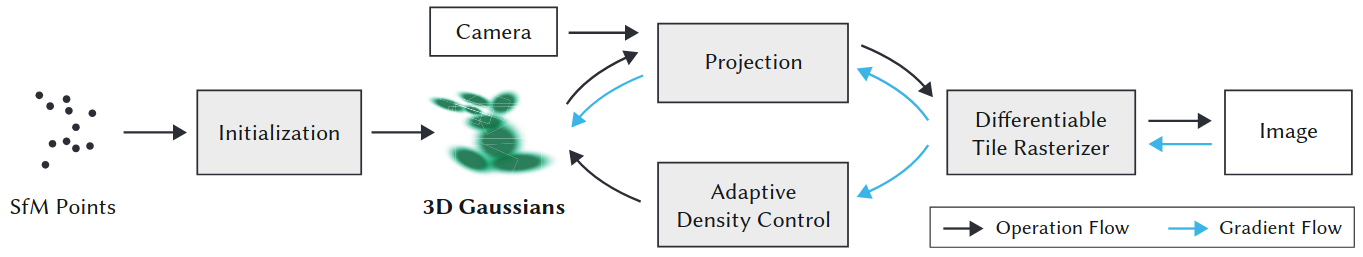
\includegraphics[width=0.7\linewidth]{figures/3dgs.png}
    \caption{Overview of the 3DGS scene optimization \cite{kerbl3Dgaussians}.}
    \label{fig:3dgspipeline}
\end{figure}

However, even though anisotropic splats are flexible in terms of the features they can model, the Gaussians fitted to the initial point cloud from SfM are usually not enough to get a good representation of the scene. This is why the authors propose a method for the adaptive control of gaussians which allows the control of the number of splats in the scene, as well as their spatial density. This mechanism identifies under-reconstructed or over-reconstructed regions through the presence of large view-space positional gradients since those areas are lacking in quality and the optimizer tries to move gaussians there to increase detail. In the case of under-reconstruction, where a single Gaussian fails to reconstruct a feature and new geometry is needed, the Gaussian is cloned and the clone is moved in the direction of the positional gradient. For over-reconstruction, usually, a Gaussian has become too big trying to cover a geometric feature, but the feature would be better modeled by a set of smaller Gaussians. In this case, the volume should be preserved but the number of entities has to increase, so the initial Gaussian is split into two smaller ones that cover the same space. In both cases, additional optimization steps are necessary to ensure that the adaptive control, has the desired effect. The disadvantage of this mechanism is that it can produce floating artifacts close to the camera, so this issue has to be addressed by pruning splats with very low opacities periodically. The two densification cases can be seen in figure \ref{fig:densification}.

\begin{figure}[H]
    \centering
    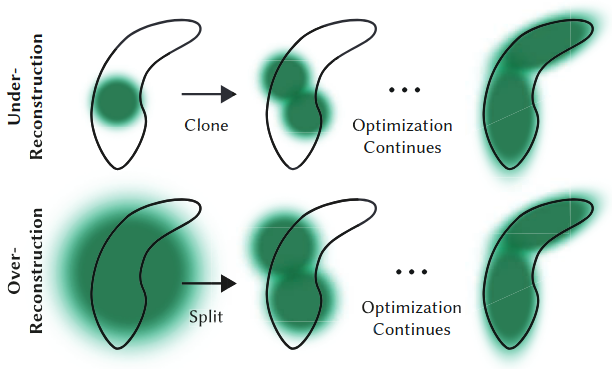
\includegraphics[width=0.6\linewidth]{figures/densification.png}
    \caption{Cases for Gaussian densification \cite{kerbl3Dgaussians}.}
    \label{fig:densification}
\end{figure}

This implementation achieves image quality metrics close to state-of-the-art, while also using a significantly faster rendering process. Additionally, since rendering is also a key part of the optimization loop, this means that the scene training times are in turn reduced compared to neural-based radiance field scene representations. 

\subsubsection{Gaussian Pruning and Compression}
The quality and rendering speed advantages of representing scenes using 3D Gaussians come with the drawback of high requirements for storage space, which is a few orders of magnitude higher than that of neural representations. LightGaussian is a method that addresses this issue through Gaussian pruning, knowledge distillation, and vector quantization of Gaussian properties in order to significantly reduce the storage requirements of these scenes with minimal impact on the rendering quality \cite{fan2023lightgaussian}. 

The standard 3DGS optimization process tends to produce dense scenes with many redundant Gaussians, which negatively impact both storage and rendering speed. Taking inspiration from neural network pruning, which removes neurons that have a low impact on the output, this method tries to identify Gaussians with a minimal contribution to the rendered images and removes them during training. Using a simplistic criterion for identifying insignificant splats, such as opacity, results in a quick degradation of the images and the loss of fine details. The authors propose a global significance score derived from the splat volume, opacity, and the number of pixels influenced over all training views. The volume is normalized by the largest 90\% of all Gaussians, otherwise, the large splats making up the background would get an exaggerated importance score. After applying the pruning process, the remaining splats will continue to be optimized, but the adaptive densification is disabled, so the number of Gaussians will not increase again.

The second strategy for reducing the size is lowering the number of spherical harmonic coefficients. In a full representation, these make up 81.3\% of the stored data. Removing them completely would decrease image quality, as they encode specular details, but in many cases, the full set of coefficients is not needed to encode all the available information. To balance model size and quality, the authors propose a knowledge distillation process, where high-degree SHs transfer the information to a lower-degree representation. The supervision of this training step is based on the difference in predicted pixel values between the two models. To increase the robustness of this process, the SH models are also sampled from synthetically generated pseudo-views, placed around the original camera positions, and following a normal distribution.

The last step proposed in this method is the Vector Quantization of spherical harmonic coefficients. This procedure is based on the assumption that a subgroup of Gaussians will exhibit a similar appearance, so they can be represented by a single encoding. After choosing the amount of desired entries in the codebook, k-means is used to create a mapping between Gaussians and their codebook entries, based on Euclidean distance in the SH vector space. Then, the codebook entries are refined without changing the mapping in order to increase visual quality. To ensure that significant details are not lost, Gaussians with a high precomputed visual importance score will not be compressed. Figure \ref{fig:lgmethod} shows an overview of the methods implemented in the LightGaussian solution.

\begin{figure}[H]
    \centering
    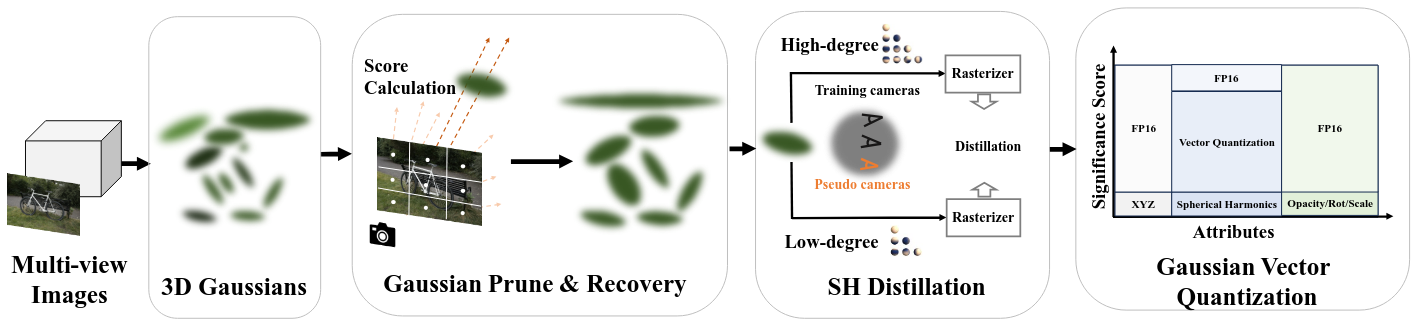
\includegraphics[width=0.8\linewidth]{figures/lgmethod.png}
    \caption{Methods implemented by LightGaussian for primitive pruning and feature compression \cite{fan2023lightgaussian}.}
    \label{fig:lgmethod}
\end{figure}

Using this approach, the authors achieve an approximated 15x reduction in storage space and over 75\% increase in FPS, while maintaining a reduction in quality under 0.4 dB PSNR. Note that the increase in rendering speed is only a result of the scene containing fewer Gaussians, as no changes have been made to optimize the renderer. 

\paragraph{}
Another publication on Gaussian scene compression achieves even better results, especially in the rendering time improvement by combining the pruning and compression with a modified rendering pipeline \cite{Niedermayr_2024_CVPR}. Unlike the previous implementation, this method does not imply a reduction in the number of Gaussians in the scene. The first step is a vector quantization of the SH coefficients and shape parameters (i. e. scale and rotation). 

Determining the quantized vectors is done by K-means clustering on the color and shape parameters separately. However, instead of using a simple Euclidean distance metric for clustering, the authors introduce a sensitivity metric.  The sensitivity of a parameter is described as the variation in image energy when a small change to the parameter is applied, summed over all the training images. This computes the gradient of image energy with respect to all parameters of all Gaussians, and it can be performed in one single backward pass. When clustering, the Euclidean distance is multiplied by the parameter's sensitivity, thus artificially pulling apart features of high sensitivity, and giving lower importance to features with low sensitivity. For color information, the top 5\% of splats in terms of sensitivity contribute most to the image, so they will not be clustered. The rest will be clustered using vector quantization. In the case of shape parameters, the clustering is done on the covariance matrices, which are afterward decomposed in a scale and a rotation matrix. Over the tested scenes, an average of 15\% of Gaussians present zero sensitivity, which means they have no contribution to the rendered image, so can in turn be pruned. 

Since quantizing parameter values comes with a cost to image quality, the scene goes through an additional stage of fine-tuning. However, instead of optimizing the individual Gaussians' parameters, the gradients are accumulated per codebook entry, and after each iteration, the quantized entries in the SH and shape codebooks are updated instead. Moreover, all Gaussian parameters except the position are quantized further to 8-bit values using the Min-Max scheme, except for position, which shows severe degradation if quantized with fewer than 16 bits. 

The last step of the compression strategy is to take advantage of the spatial coherency of reconstructed scenes, where Gaussians in close proximity to one another are expected to have similar, or even the same, properties. By ordering the Gaussians according to a Z-order curve in Morton order, the performance of the LZ77 run-length encoding can be improved. Since the Gaussian properties have been quantized, the final compression also uses Huffman coding to take advantage of the lower entropy of the information.

\begin{figure}[H]
    \centering
    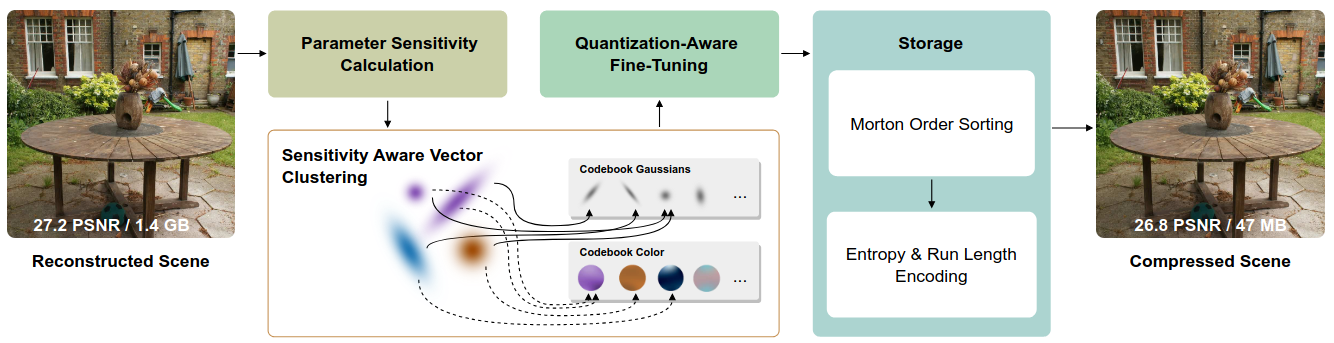
\includegraphics[width=0.8\linewidth]{figures/compression.png}
    \caption{Gaussian compression pipeline \cite{Niedermayr_2024_CVPR}.}
    \label{fig:compression}
\end{figure}

Besides the compression strategy shown in figure \ref{fig:compression}, this method also proposes a modified rendering pipeline. The first step remains the same as in the original 3DGS implementation, projecting the Gaussian into splats on screen, eliminating splats that are not visible, computing the color from the SH coefficients, and ordering them by depth. However, instead of using a tiling software rasterizer, this implementation uses the traditional GPU rendering pipeline. For each splat on the screen, a quad made up of two triangles is instantiated. The vertex shader computes for each splat the vertex position, such as the quad covers the 99\% confidence area of the Gaussian. Then, it outputs to the fragment shader the solid splat color and the Gaussian's center. Then, the pixel shader uses the distance from the splat center to compute the exponential color and opacity falloff and perform the blending into the framebuffer. 

Using this strategy, the method achieves an average 26x compression over all scenes with an average quality loss of 0.26dB PSNR. The rasterization pipeline also sees a 4x improvement in speed. Approximately a 2x increase in rendering performance can be attributed to the lower bandwidth requirements of the compressed splat representation, and the additional improvement is a result of using the more efficient hardware rasterization pipeline, instead of using a software rasterizer. 

\paragraph{}
Another attempt at making Gaussian scenes smaller uses a learnable approach to both pruning and color encoding \cite{Lee_2024_CVPR}. The number of Gaussians in the scene is controlled by a learnable mask. Instead of waiting for the entire training process to end before pruning, this method eliminates splats based on a volume mask after each densification step. The learnable mask is based on the volume and opacity of Gaussians, since these two metrics define a Gaussian's expected contribution to the rendered image. The balance between the eliminated Gaussians and the rendering quality is maintained by introducing an additional masking loss term in the optimization function. The advantage of this masking procedure is that it also reduces the number of primitives during training, resulting in lower memory requirements compared to the original 3DGS. Encoding the geometric properties of scale and rotation quaternions is done using residual vector quantization, where the number of cascading stages is chosen to balance performance and quality. 

Instead of encoding the color information in a similar codebook, this implementation uses a hash grid followed by a small multi-layer perceptron model to estimate color from the viewing direction. The Gaussian center is fed as input to the hash grid, then the resulting features and the camera viewing direction are used as input to the MLP to get the color estimate. Of course, the unbounded coordinates of the scene have to be bounded first using a technique similar to Mip-NeRF360. This implicit representation allows for very good compression since the SH coefficients take up most of the storage space.

\begin{figure}[H]
    \centering
    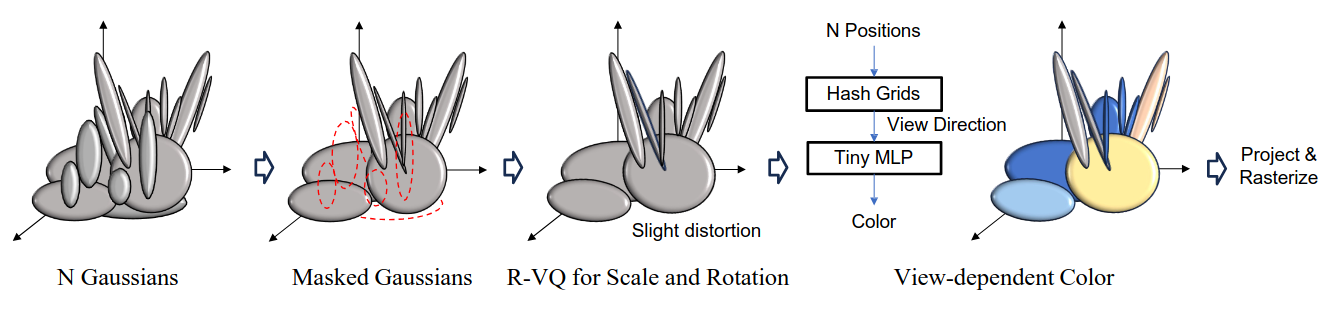
\includegraphics[width=0.7\linewidth]{figures/compact_arch.png}
    \caption{Details of the compact Gaussian architecture \cite{Lee_2024_CVPR}.}
    \label{fig:compact_arch}
\end{figure}

Using this masking and encoding approach shown in figure \ref{fig:compact_arch}, this method achieves up to 22x storage compression, but usually without a loss in quality, and many times with an increase in observed PSNR compared to the reference implementation, hinting that the masking process might also be beneficial for reconstruction quality, not only for space optimization.

\paragraph{}
\textit{Scaffold-GS} introduces a hybrid scene representation by implicit encoding of Gaussian properties through an MLP and an explicit representation of feature anchor points in the scene for Gaussian distribution \cite{scaffoldgs}. The initial point cloud produced by COLMAP is used to produce a sparse grid of anchor points, where each anchor tethers a set of neural Gaussians with learnable properties. This approach leverages the structural information given by the point cloud by allowing the Gaussians to only optimize locally, thus reducing drift and "floater" artifacts. 

For each anchor point, \textit{k} neural Gaussians are spawned, each being defined by a 3D offset from the anchor point location. Each anchor is also assigned a feature bank of 32 components and a scaling factor. A set of very small MLPs is then optimized to estimate opacity, color, quaternions, and scales for each of the \textit{k} spawned Gaussians based on the viewing direction, camera distance, and the feature bank specific to each anchor. The offsets and scaling factors for each anchor are also learnable parameters. Only visible anchor points are evaluated through the MLP, thus reducing the overhead. It is worth mentioning that, even though there are separate MLPs for estimating the different properties, these are global to the scene, and not instantiated per anchor point.

The point cloud from SfM gives a good starting point for creating the anchor grid cells. However, some areas of the scene need more detail than can be provided by the set of \textit{k} Gaussians that can be produced by a single anchor. To determine such cases, neural Gaussian gradients for each cell are accumulated over multiple training iterations, and if they exceed a set threshold, the cell will go through a densification process. This involves spawning new anchor points in a multi-resolution grid based on the initial scaffold cells. To regulate this densification process, trivial Gaussians are identified by their opacity. If an anchor cannot produce Gaussians with opacity high enough, the respective anchor is pruned from the structure.

\begin{figure}[H]
    \centering
    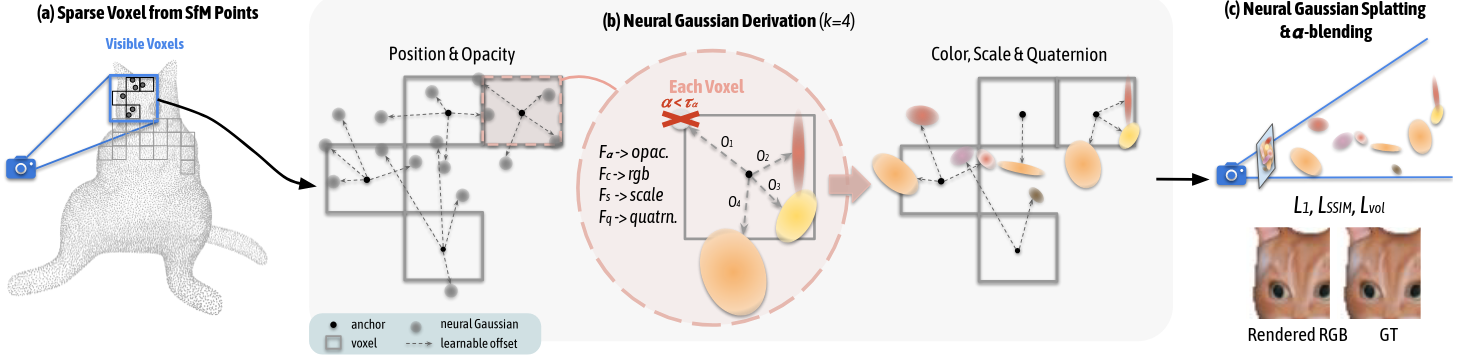
\includegraphics[width=0.8\linewidth]{figures/scaffoldgs.png}
    \caption{Scaffold-GS optimization pipeline \cite{scaffoldgs}.}
    \label{fig:scaffold}
\end{figure}

This implementation, also shown in figure \ref{fig:scaffold} achieves a slight increase in rendering quality and speed compared to the reference 3DGS, and a reduction between 3.8x to 10.2x in required memory thanks to the implicit representation of Gaussian parameters. Additionally, it showcases better view adaptability to camera positions outside of the training poses.

\subsubsection{Gaussian Splatting Anti-Aliasing}
While a lot of research goes into optimizing the storage size and rendering speeds of Gaussian models, some implementations focus more on the image quality aspects of this kind of environment representation. One clear issue is the lack of regularization with respect to the sampling frequency during training, which leads to aliasing artifacts and high-frequency noise \cite{Yu2024MipSplatting}. The MipSplatting implementation aims to address these issues through two separate mechanisms. Their approach is mainly based on the Nyquist-Shannon sampling theorem \cite{nyquist}, which states that in order to correctly reconstruct a continuous signal from discrete samples without losing information, the original signal has to be band-limited, and the sampling frequency should be at least twice the maximum frequency of the continuous signal. In the case of 3DGS scenes, the spatial sampling frequency is given by the camera intrinsics, as well as its position relative to the scene. This means that Gaussians are sampled differently depending on the view, and the reconstruction does not account for views outside the training camera positions. In the reference implementation, projected splats that are thinner than one pixel are dilated by an arbitrarily chosen kernel, which ensures that all visible splats have a contribution on screen. However, this leads the optimizer to favor the creation of thin Gaussians and underestimates their real scale. This works for the training images but leads to erosion and dilation artifacts when the camera moves closer or further away from the scene, or the sensor resolution changes. Figure \ref{fig:mipsplat_degen} illustrates these kinds of artifacts.

\begin{figure}[H]
    \centering
    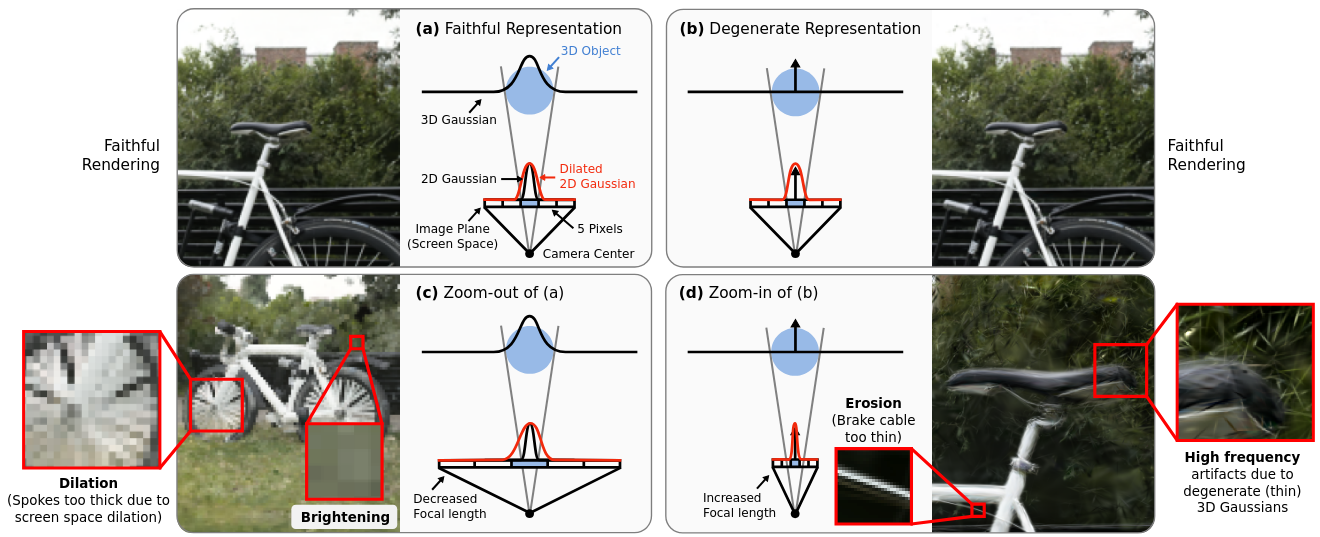
\includegraphics[width=0.8\linewidth]{figures/mipsplat_degen.png}
    \caption{Dilation and erosion artifacts appear when the sampling frequency differs from the training cameras \cite{Yu2024MipSplatting}.}
    \label{fig:mipsplat_degen}
\end{figure}

The first change the authors propose to mitigate these issues is regularizing the Gaussian spatial frequency during training. The first step is to determine the maximal sampling frequency of each Gaussian, taking into account all training images, distance to the camera, and focal length. This process is done at set intervals during training. Then, for each Gaussian, a 3D low-pass filter is applied, with the cutoff frequency set at the maximal sampling frequency for that Gaussian. This operation is done before projecting to screen-space, by the convolution of the initial Gaussian with the Gaussian low-pass filter. Using this filter solves the issue of high-frequency artifacts in reference images, but aliasing still appears when rendering the scene in lower resolution.

The second modification comes in the form of replacing the dilation mechanism in the final pre-processing stage with a 2D Mip filter. This is based on the physical principle of a camera capturing light, where the photons are integrated over the area of a pixel. A good estimation of this process would be applying a 2D box filter in image space, but this would require filtering all projected splats after they are rasterized, but before they are blended into the framebuffer to produce the final image. A more efficient way to achieve a similar effect is to a 2D Gaussian filter to each splat before rasterization, as this process only involves operating on the covariance matrix.

Applying the steps above to the training and rendering routines respectively, this implementation achieves slightly improved quality metrics when generating full-resolution images, but it retains more detail and achieves an increase of around 1 to 2 dB PSNR when decreasing the sampling resolution.
\paragraph{}
Another proposed solution to the issues above is to create a multi-scale representation of the scene, and select the Gaussians to be rendered based on the estimated sampling frequency \cite{yan2024multiscale3dgaussiansplatting}. The implementation creates a 4-tier representation, where each level is optimized at 1x, 4x, 16x, and 64x downsampled resolution respectively. The Gaussians at coarser levels are created by merging fine-level Gaussians, and at render-time, the selection for render is done by each primitive's pixel coverage. The pixel coverage metric is defined by the length, in pixels, of the shortest axis of the Gaussian.

The scene is initialized using the same strategy as the reference implementation and it goes through the same optimization process in the first phase, including the densification process. Then, the images are rendered at the downsampled resolutions, and the splats that fall below a predefined pixel coverage metric are marked for aggregation into the next level. The aggregation process is done by dividing the space into a grid sized according to the downsampling rate, and merging the Gaussians in each cell in order to form a new Gaussian for the next resolution level. The aggregation is done by average pooling of all the parameters that define the primitives. After all levels are generated, the optimization process continues using images at all resolutions mentioned above, in order to fit all the multi-resolution levels to the reference images.
For each Gaussian, a minimum and maximum pixel coverage threshold is stored, which are then used in rendering to decide which Gaussians in the hierarchy should be passed for rasterization. Figure \ref{fig:multiscale_aggregate} shows an overview of this pipeline.

\begin{figure}[H]
    \centering
    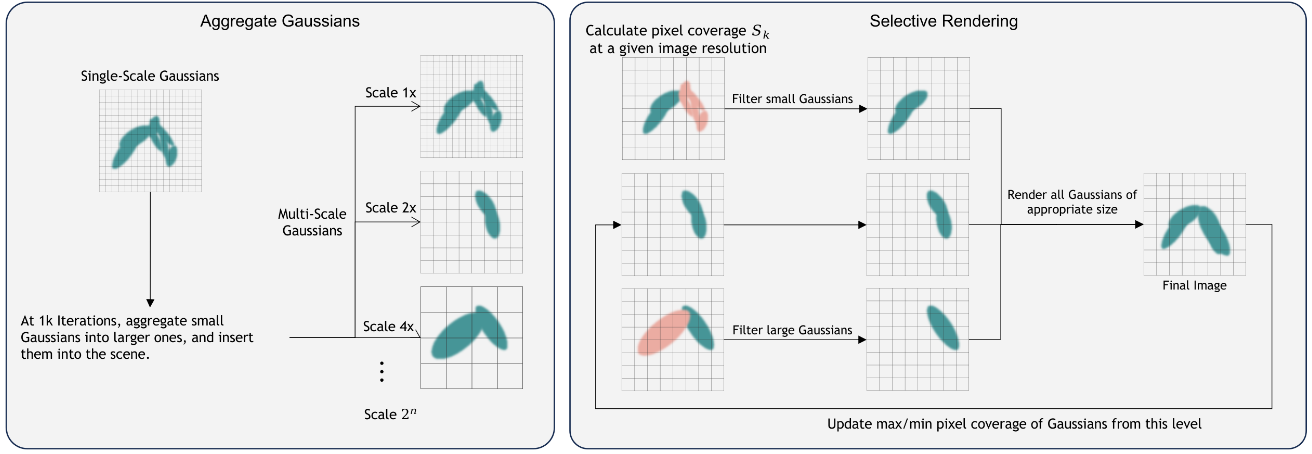
\includegraphics[width=0.8\linewidth]{figures/multiscale_gaussian.png}
    \caption{Overview of the training pipeline, including the multiscale aggregation of primitives and the selective rendering process \cite{yan2024multiscale3dgaussiansplatting}.}
    \label{fig:multiscale_aggregate}
\end{figure}

Since not all primitives are small enough to be aggregated, the whole process increases the Gaussian count by an average of 5\% in order to create the three additional resolution levels. The render quality benefits of this method increase as the render resolution decreases, offering an increase of between 13\% and 66\% in PSNR and 140\% to 2400\% improvement in rendering time. The improvement in rasterization speed comes from the implementation of the tiling rasterizer: at lower resolution, each tile overlaps more splats, so the same thread workgroup has to process more primitives. In the reference implementation, decreasing the rendering resolution or moving away from the scene in such a way that the scene occupies less space on the screen results in an increase in rendering times, which this implementation solves by reducing the number of primitives as they occupy less space on the screen. 

\subsubsection{Multi-resolution Gaussian Representations}
As discussed before, Gaussian scenes have the disadvantage of large memory requirements when compared to neural representations. The research discussed above focuses on reducing this requirement for benchmark scenes, however, another problem is posed by the reconstruction of very large environments, such as cityscapes, which many times will not fit the memory limitations of even workstation-grade GPUs. To overcome this limitation, most implementations use a combination of space partitioning schemes and multi-resolution representation to enable training and rendering of these massive scenes.

GityGaussian \cite{liu2024citygaussian} proposes an implementation based on a divide-and-conquer strategy and multiple levels of detail to facilitate training large-scale 3DGS environments. The scene is first partitioned into adjacent blocks that can be optimized in parallel, thus reducing the memory strain on each GPU. Individual block training, however, poses the issue of "floater" artifacts which try to represent the space outside the training block that is seen by the cameras. This leads to inaccurate representation and makes combining the blocks after training more difficult. This is why the initial point cloud produced by COLMAP is used to produce a scene prior of the entire environment, which is a coarse Gaussian representation of the model. Because the number of Gaussians remains relatively low, this training step can be done before the partitioning. Using a scene prior proved to produce much better reconstructions and allows for seamless merging of blocks. Because the scenes this method is aimed at are usually unbounded, a linear contraction of the space allows for a more even distribution of primitives inside blocks and avoids almost empty blocks. Then, for each block, the camera poses that capture that block need to be registered. To determine this registration, an SSIM loss is computed between the fully rendered image and the image rendered without that block, and if the loss exceeds some threshold, the block is considered to have a considerable contribution to that pose. Then, each block is trained individually from its respective camera poses, using the scene prior for rendering but only performing fine-tuning on the primitives inside the block. Then, the complete fine-tuned model can be obtained from the direct concatenation of the blocks. Figure \ref{fig:city_training} shows the block training process, including the partitioning and the scene prior.

\begin{figure}[H]
    \centering
    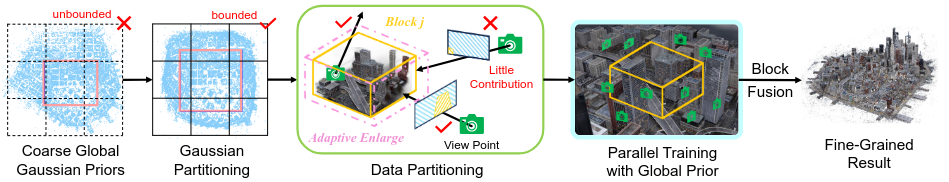
\includegraphics[width=0.8\linewidth]{figures/citygs_training.png}
    \caption{CityGS block optimization pipeline \cite{liu2024citygaussian}.}
    \label{fig:city_training}
\end{figure}

The level-of-detail component of this implementation uses the same mechanism as the one proposed in LightGaussian \cite{fan2023lightgaussian}, in order to reduce the number of primitives successively across multiple detail levels. Because lover-detail levels are used for blocks further away from the camera, where high-frequency details become more insignificant, the decrease in quality is less noticeable. During rendering, the selection of which level to rasterize is done based on each block's distance to the camera, only for the blocks that intersect the frustum, as shown in figure \ref{fig:city_render}. In practice, the extent of many blocks is artificially enlarged by floaters, so the authors propose an approach based on the Median Absolute Deviation algorithm \cite{dodge2008concise} to compute block bounds more accurately.

\begin{figure}[H]
    \centering
    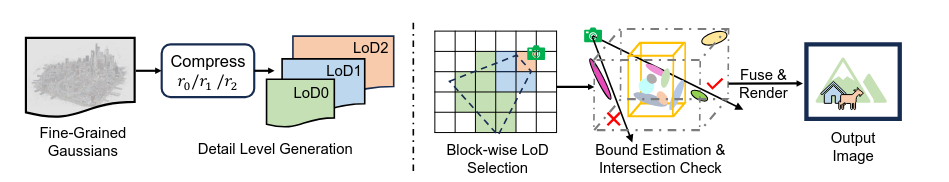
\includegraphics[width=0.8\linewidth]{figures/citygs_rendering.png}
    \caption{CityGS rendering process, including the selection of the appropriate LoD \cite{liu2024citygaussian}.}
    \label{fig:city_render}
\end{figure}

The tests were performed on the \textit{MatrixCity} \cite{li2023matrixcity} dataset, which is a synthetic, large-scale collection of cityscape images. Compared to the reference 3DGS implementation, CityGaussian achieves an increase of 3.79 dB PSNR, as it is able to generate more Gaussian primitives for a better scene representation, and more than doubles the rendering speed through the use of the LoD structure. 

\paragraph{}
Coming as an extension to Scaffold-GS, OctreeGS takes advantage of the multiresolution grids that are generated in the densification process when more anchors are spawned in order to build an octree structure \cite{ren2024octreegs}. The octree is not generated from a single root node, but it starts from the grid generated on the SfM point cloud. In this implementation, a level of detail corresponds to a level in the octree. Initially, the anchors are associated with all LoDs, and each anchor can be rendered at a different detail level. The selection for the appropriate level during rendering is based on the degree of complexity in that area of the scene and the distance between the anchor point and the camera. 

Similar to the method that it is based on, this implementation uses grid cell gradients to drive anchor densification. Even though all detail levels start off with the same set of anchors, the densification will be performed differently based on the level. Starting from the gradient threshold defined by Scaffold-GS, a set of additional, increasingly higher thresholds are generated. These values are used to decide, based on the gradient magnitude, which level the new anchor should be spawned in. Higher gradients mean that the anchor will be assigned to a finer detail level. This restricts the anchors from growing too aggressively into the finer levels. Anchor pruning uses the same strategy as Scaffold-GS, removing anchors that fail to produce sufficiently opaque Gaussians.

Training is done in a coarse to fine manner, first optimizing the lowest level of detail, and then enabling the optimizer to spawn anchors into the higher levels one by one. As mentioned before, besides camera distance, scene detail is also a driving factor for LoD selection. To encode this metric, a learnable render bias is assigned to each anchor, which then influences the level selection. Using this bias, anchors close to the camera can be assigned a low detail level if they do not represent complex features, and anchors further away can get a higher level if they contain a lot of detail that contributes a lot to the render. However, these biases are learnable parameters that are optimized to lower the training objective function, so they might not be exactly and only determined by anchor detail complexity. 

\begin{figure}[H]
    \centering
    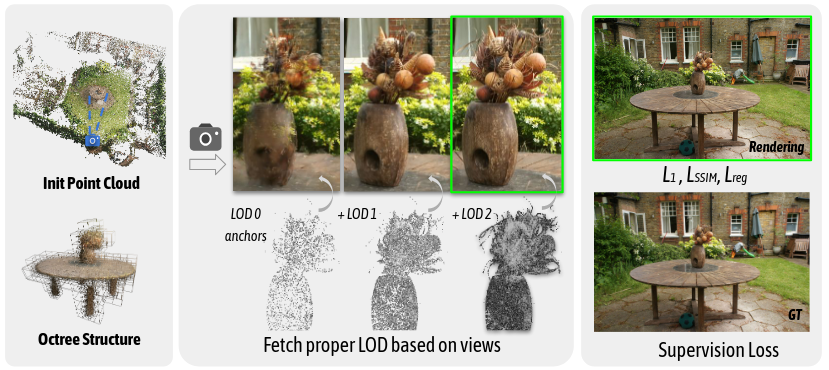
\includegraphics[width=0.8\linewidth]{figures/octreegs.png}
    \caption{Traning pipeline starting from the sparse point data, to LoD generation and selection \cite{ren2024octreegs}. The procedure inside each node is similar to ScaffoldGS.}
    \label{fig:octreegs_pipeline}
\end{figure}

This method, also illustrated in figure \ref{fig:octreegs_pipeline}, provides an image quality increase when the scene is rendered at a lower resolution (i.e., the camera is far away from part of the scene), however, its main advantage is the ability to render complex scenes at real-time 45-47 FPS, while other methods such as Mip-Splatting (10-12 FPS) and Scaffold-GS (3-5 FPS) fail to reach a 30FPS consistent rendering speed.

\paragraph{}
The authors of the reference 3DGS implementation also provide a solution for optimizing and rendering massive environments through a hierarchical LoD structure \cite{kerbl_hierarchy}. Creating a tree-based hierarchy for the levels of detail allows different parts of the environment to be rendered at different complexities while also having good granularity when transitioning between the levels. The proposed structure contains the original Gaussians as the leaves of the tree, and merged primitives in the intermediary nodes. In order to not overly complicate the existing pipeline, the merged primitives are also 3D Gaussians. This poses the problem of merging two Gaussians into one while maintaining the aspect as close as possible to the original. The proposed solution uses a weighted average for the mean and SH coefficients, while the merged covariance takes into account both the initial covariances and the means. The weights are defined by each Gaussian's contribution to the image, which is given by the opacity and the surface area of the ellipsoid defined by the Gaussian distribution. The opacity of a merged Gaussian sometimes has a slower fall-off, so it is allowed to go over 1 and is only clamped at 1 during rendering.

Having the strategy for merging two 3D Gaussians, the next problem is finding candidates for merging. The implementation proposes a BSP partitioning of the space starting from the axis-aligned bounding box of the entire scene as the root node. Then, the volume is divided into two children by a median split. This means that the Gaussians are projected on the longest axis of the bounding box, then the split is performed at the median projection, such that the two resulting will have an equal number of Gaussians (pr differ by one in the case of an odd number of primitives). This process is performed recursively until each bounding box only contains one Gaussian. Then, starting from the leaves, the Gaussians are merged in the interior nodes towards the root. Because this is a binary tree, primitives will always be merged two at a time, even if they are in turn merged representations of other Gaussians.

During rendering, a target node granularity is set depending on the required quality. Then, the problem of selecting the proper level for rendering becomes one of finding a graph cut where all the nodes satisfy the granularity condition, which is determined by evaluating the size of the node's bounding box projection on the screen, as shown in figure \ref{fig:inria_granularity}. Traversing the structure from the root, when a parent node does not satisfy the granularity, but the child satisfies it, the child will be selected into the graph cut. For smooth transitions, the authors propose an interpolation method between parent and children primitives to reduce popping artifacts when transitioning between levels.

\begin{figure}[H]
    \centering
    \begin{minipage}{0.45\textwidth}
       \centering
        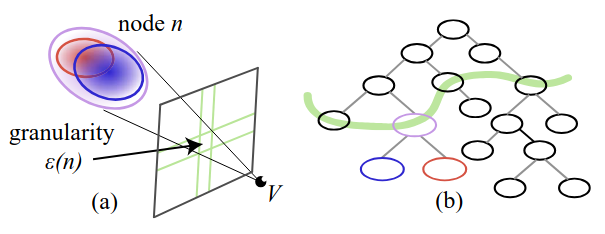
\includegraphics[width=\linewidth]{figures/inria_granularity.png}
        \caption{Node granularity computation and the respective graph cut for a target granularity \cite{kerbl_hierarchy}.}
        \label{fig:inria_granularity}
    \end{minipage}\hfill
    \begin{minipage}{0.45\textwidth}
        \centering
        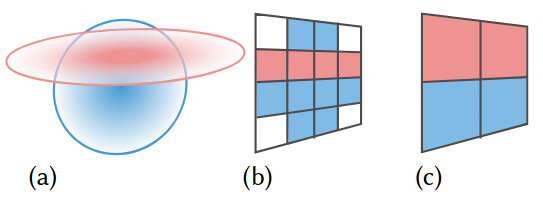
\includegraphics[width=\linewidth]{figures/inria_train.png}
        \caption{Two nodes in the scene tree (a), and their rasterization at two different target granularities (b and c).}
        \label{fig:inria_train}
    \end{minipage}
\end{figure}

For training, the scene is optimized at multiple granularity levels, as illustrated in figure \ref{fig:inria_train}, which allows the merged intermediary Gaussians to also be trained against the full-resolution reference images. This solution is particularly useful when dealing with large scenes. In that case, the scene is split into chunks, each one having its individual LoD hierarchy. A coarse scene prior is first trained and used to represent the environment outside each chunk. The chunks are then consolidated in the final scene. 

When evaluated against other methods on chunk-sized scenes, the quality improvements over the reference implementation are small. However, on the SmallCity and Campus datasets, it manages to achieve a consistent 30+ FPS at a 3-pixel granularity, while those scenes would not even be able to be optimized or rendered by the original 3DGS due to their size. However, these results were collected on an NVIDIA A6000 GPU.